\documentclass[tikz,border=6pt]{standalone}
\usepackage{tikz}
\usetikzlibrary{calc}

\begin{document}
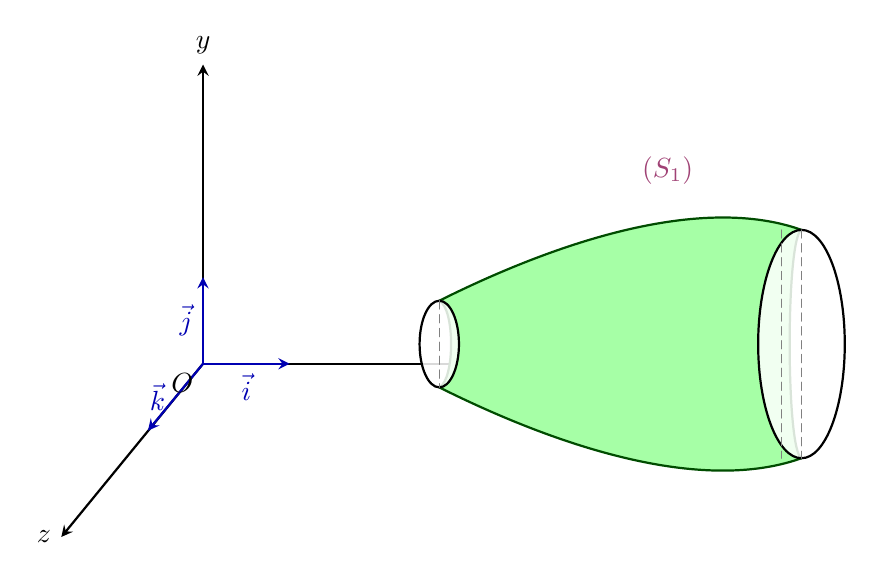
\begin{tikzpicture}[line cap=round,line join=round,>=stealth,scale=1]

% -----------------------
% Axes
% -----------------------
\draw[->,thick] (0,0) -- (6.2,0) node[below right] {$x$};
\draw[->,thick] (0,0) -- (0,3.8) node[above] {$y$};
\draw[->,thick] (0,0) -- (-1.8,-2.2) node[left] {$z$};

% Unit vectors i, j, k
\draw[->,blue!70!black,thick] (0,0) -- (1.1,0) node[midway,below] {$\vec i$};
\draw[->,blue!70!black,thick] (0,0) -- (0,1.1) node[midway,left] {$\vec j$};
\draw[->,blue!70!black,thick] (0,0) -- (-0.7,-0.85) node[midway,left] {$\vec k$};

\node[below left] at (0,0) {$O$};

% -----------------------
% "Surface" verte (tube)
% -----------------------
% Paramètres visuels
\def\xL{3.0}   % x de la section gauche
\def\xR{7.6}   % x de la section droite
\def\yC{0.25}  % centre vertical du tube
\def\aL{0.25}  % demi-axe horizontal ellipse gauche
\def\bL{0.55}  % demi-axe vertical ellipse gauche
\def\aR{0.55}  % demi-axe horizontal ellipse droite
\def\bR{1.45}  % demi-axe vertical ellipse droite

% Corps du tube (haut / bas en courbes de Bézier)
\path
  (\xL,\yC+\bL)
    .. controls (\xL+1.2,\yC+\bL+0.6) and (\xR-1.4,\yC+\bR+0.5) ..
  (\xR,\yC+\bR)
    .. controls (\xR-0.2,\yC+\bR-0.1) and (\xR-0.2,\yC-\bR+0.1) ..
  (\xR,\yC-\bR)
    .. controls (\xR-1.4,\yC-\bR-0.5) and (\xL+1.2,\yC-\bL-0.6) ..
  (\xL,\yC-\bL)
    .. controls (\xL+0.2,\yC-\bL+0.1) and (\xL+0.2,\yC+\bL-0.1) ..
  (\xL,\yC+\bL)
  coordinate[pos=0] (dummy);

% Remplissage + contour
\fill[green!35] 
  (\xL,\yC+\bL)
    .. controls (\xL+1.2,\yC+\bL+0.6) and (\xR-1.4,\yC+\bR+0.5) ..
  (\xR,\yC+\bR)
    .. controls (\xR-0.2,\yC+\bR-0.1) and (\xR-0.2,\yC-\bR+0.1) ..
  (\xR,\yC-\bR)
    .. controls (\xR-1.4,\yC-\bR-0.5) and (\xL+1.2,\yC-\bL-0.6) ..
  (\xL,\yC-\bL)
    .. controls (\xL+0.2,\yC-\bL+0.1) and (\xL+0.2,\yC+\bL-0.1) ..
  cycle;

\draw[thick,green!30!black]
  (\xL,\yC+\bL)
    .. controls (\xL+1.2,\yC+\bL+0.6) and (\xR-1.4,\yC+\bR+0.5) ..
  (\xR,\yC+\bR)
    .. controls (\xR-0.2,\yC+\bR-0.1) and (\xR-0.2,\yC-\bR+0.1) ..
  (\xR,\yC-\bR)
    .. controls (\xR-1.4,\yC-\bR-0.5) and (\xL+1.2,\yC-\bL-0.6) ..
  (\xL,\yC-\bL)
    .. controls (\xL+0.2,\yC-\bL+0.1) and (\xL+0.2,\yC+\bL-0.1) ..
  cycle;

% Section droite (ellipse "face")
\fill[white,opacity=0.85] (\xR,\yC) ellipse [x radius=\aR, y radius=\bR];
\draw[thick]              (\xR,\yC) ellipse [x radius=\aR, y radius=\bR];

% Section gauche (petite ellipse)
\fill[white,opacity=0.85] (\xL,\yC) ellipse [x radius=\aL, y radius=\bL];
\draw[thick]              (\xL,\yC) ellipse [x radius=\aL, y radius=\bL];

% Génératrice pointillée interne (comme sur l’image)
\draw[densely dashed,gray]
  ($( \xR,\yC ) + (0, \bR)$) -- ($( \xR,\yC ) + (0,-\bR)$);
\draw[densely dashed,gray]
  ($( \xL,\yC ) + (0, \bL)$) -- ($( \xL,\yC ) + (0,-\bL)$);

% Petit repère de "profondeur" en pointillés dans la face droite
\draw[densely dashed,gray]
  ($( \xR,\yC ) + (-0.25, \bR)$) -- ($( \xR,\yC ) + (-0.25,-\bR)$);

% Label (S1)
\node[magenta!60!black] at (5.9,2.45) {$(S_1)$};

\end{tikzpicture}
\end{document}
